\section{2D-LiDARとYOLOv5を用いた手法}
飯田一成らの論文\cite{深層学習を用いた人追従機能の開発}では、
リアルタイム物体検出アルゴリズムであるYOLOv5を用いて、2D-LiDARの距離データから
人の脚部を検出している。\\ \indent
提案手法は、\ref{2-1_Image of centroid}のように2D-LiDARの距離データを画像化し、学習したYOLOv5の物体検出により画像から
人の脚部を検出する。複数検出する場合があるため、検出する範囲を一定の位置に設定している。
また、衝突\\ \indent
実験方法は、追従実験と衝突回避実験がある。追従実験ではFig. \ref{2-1_Data Acquisition Environment} 3つの経路を設定し、1回のみの試行である。
衝突回避実験では、人追従中に追従対象者とロボットとの間に障害物を設置し、停止したかを
3つの状況に分けてそれぞれ10回試行している。実験結果は、追従実験では3つの経路において20[m]
の人追従ができていたが、雑多な環境下では追従中に停止することがあった。
衝突回避実験ではTable \ref{2-1_Success rate of emergency stops on each road}
に示すように、すべての試行において衝突回避ができていた。\\ \indent
飯田一成らの手法では、雑多な環境下での追従が停止することが実験結果として挙げられており、
課題としてYOLOv5の学習に使用するデータセットや学習モデルの改良が挙げられている。
また、歩行速度の課題として、より速い歩行速度へ追従するため、ロボット台車の制御手法の改良
が挙げられている。

\begin{figure*}[h]
  \begin{center}
  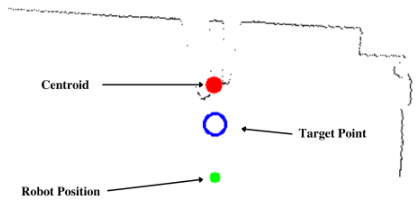
\includegraphics[height=60mm,clip]{figure/2-1_Image-of-centroid.png}
  \caption{Image of centroid\cite{深層学習を用いた人追従機能の開発}}
  \label{2-1_Image of centroid}
  \end{center}
\end{figure*}

\begin{figure*}[h]
  \begin{center}
  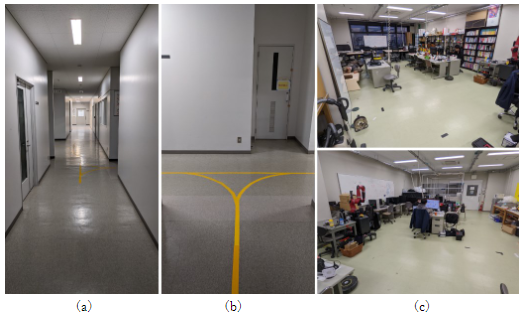
\includegraphics[height=60mm,clip]{figure/2-1_Data-Acquisition-Environment.png}
  \caption{Data Acquisition Environment\cite{深層学習を用いた人追従機能の開発}}
  \label{2-1_Data Acquisition Environment}
  \end{center}
\end{figure*}

\begin{table}[h]
  \begin{center}
    \caption{{Success rate of emergency stops on each road\cite{深層学習を用いた人追従機能の開発}}
    \label{2-1_Success rate of emergency stops on each road}}
    \scalebox{1.0}[0.9]{
      \begin{tabular}{c|ccc} \hline
        \multicolumn{1}{c|}{} & \multicolumn{3}{c}{Distance between robot and obstacle} \\
        \cline{2-4}
        \multicolumn{1}{c|}{}
          & 0.1[m] & 0.2[m] & 0.3[m] \\ \hline
          Straight road & 100[\%] & 100[\%] & 100[\%] \\
          Curved road & 100[\%] & 100[\%] & 100[\%] \\
          Miscellaneous road & 100[\%] & 100[\%] & 100[\%] \\ \hline
      \end{tabular}
    }
  \end{center}
\end{table}
\clearpage
\section{2D-LiDARの距離データをクラスタリングする手法}
Fei Luoらの研究\cite{Temporal convolutional networks for multi-person activity recognition using a 2D LIDAR}
では、キッチン内を想定し、人が歩行した軌跡のクラスタリングを行っている。\\ \indent
提案手法は、Fig. \ref{2-2_LIDAR data processing}が処理の全体像である。Fig. \ref{2-2_LIDAR data processing}
(a)では、2D-LiDARから提供される距離データをプロットしている。Fig. \ref{2-2_LIDAR data processing}(b)
では、密度ベースのクラスタリングアルゴリズムである
DBSCAN (Density-Based Spatial Clustering of Applications with Noise)
を用いて距離データをクラスタリングする。\ref{2-2_LIDAR data processing}(c)では、
Fig. \ref{2-2_Human recognition}のように定義した幾何学的特徴をもとにランダムフォレストにより、
人間と非人間の2つに分類する。Fig. \ref{2-2_LIDAR data processing}(c)では、カルマンフィルタを用いて
人間が移動した軌跡を生成し、ガウスノイズなどの軌跡拡張が行われ、
LSTM (Long Short-Term Memory)とTCN (Temporal Convolutional Network)の両方に入力される。
活動クラスに分類される。LSTMは、時間経過に伴って変化するデータを学習できる
RNN(Recurrent Neural Network)の勾配消失問題を解消したものであり、TCNは時系列データに対して
CNN (Convolutional Neural Network)を用いているものである。\\ \indent
実験方法は、学習したLSTMとTCNを用いて、Fig. \ref{2-2_Kitchen scenario}のような環境において
15種類の歩行パターンを分類させ、LSTMとTCNの分類精度の評価を行う。
実験結果はTable \ref{2-2_THE EFFECT OF TRAJECTORY AUGMENTATION}のようになっており、
LSTMよりTCNのほうが分類精度が高いことが明らかになっている。\\ \indent
Fei Luoらの手法では、人の脚部が幾何学的特徴からの検出であり、脚部に類似している物体が
乱雑に配置されていた場合、人の脚部であると誤検出されてしまう課題が考えられる。

\begin{figure*}[h]
  \begin{center}
  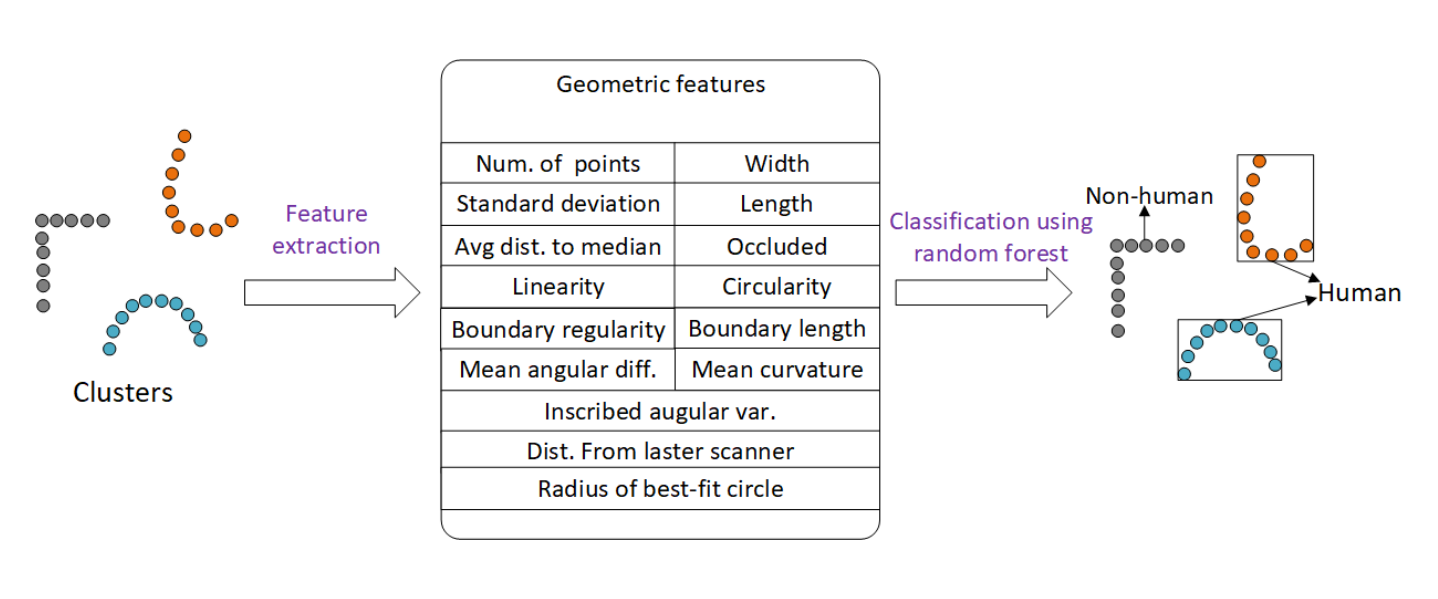
\includegraphics[height=70mm,clip]{figure/2-2_Human-recognition.png}
  \caption{Human recognition\cite{Temporal convolutional networks for multi-person activity recognition using a 2D LIDAR}}
  \label{2-2_Human recognition}
  \end{center}
\end{figure*}

\begin{figure*}[h]
  \begin{center}
  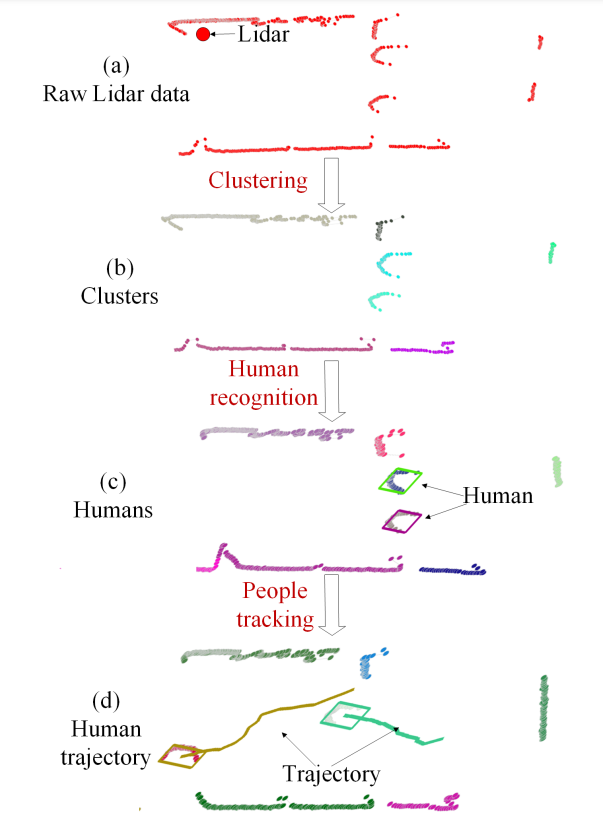
\includegraphics[height=100mm,clip]{figure/2-2_LIDAR-data-processing.png}
  \caption{LIDAR data processing\cite{Temporal convolutional networks for multi-person activity recognition using a 2D LIDAR}}
  \label{2-2_LIDAR data processing}
  \end{center}
\end{figure*}

\begin{figure*}[h]
  \begin{center}
  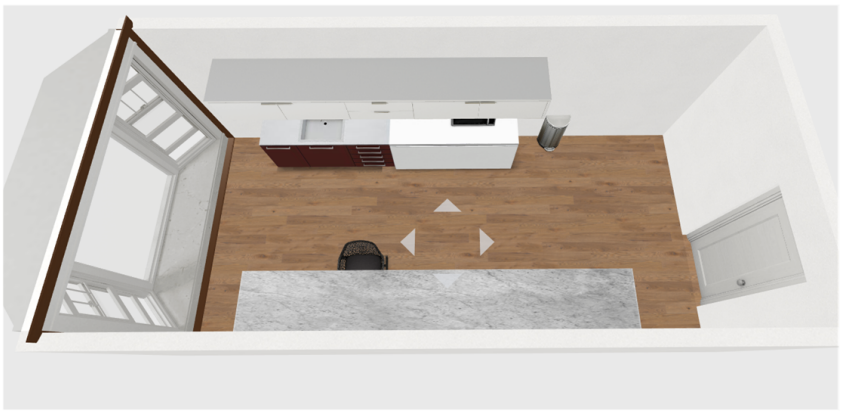
\includegraphics[height=50mm,clip]{figure/2-2_Kitchen-scenario.png}
  \caption{Kitchen scenario\cite{Temporal convolutional networks for multi-person activity recognition using a 2D LIDAR}}
  \label{2-2_Kitchen scenario}
  \end{center}
\end{figure*}

\begin{table}[b]
  \begin{center}
    \caption{{THE EFFECT OF TRAJECTORY AUGMENTATION\cite{Temporal convolutional networks for multi-person activity recognition using a 2D LIDAR}}
    \label{2-2_THE EFFECT OF TRAJECTORY AUGMENTATION}}
    \scalebox{1.0}[0.9]{
      \begin{tabular}{l|c|c|c} \hline
        & OA & Recall & F1 \\ \hline
        TCN with trajectory augmentation & 99.49\% & 99.53\% & 99.51\% \\ \hline
        TCN without trajectory augmentation & 97.96\% & 97.93\% & 97.96\% \\ \hline
        LSTM with trajectory augmentation & 99.39\% & 99.41\% & 99.39\% \\ \hline
        LSTM without trajectory augmentation & 97.65\% & 97.79\% & 97.65\% \\ \hline
      \end{tabular}
    }
  \end{center}
\end{table}